
\cleardoublepage

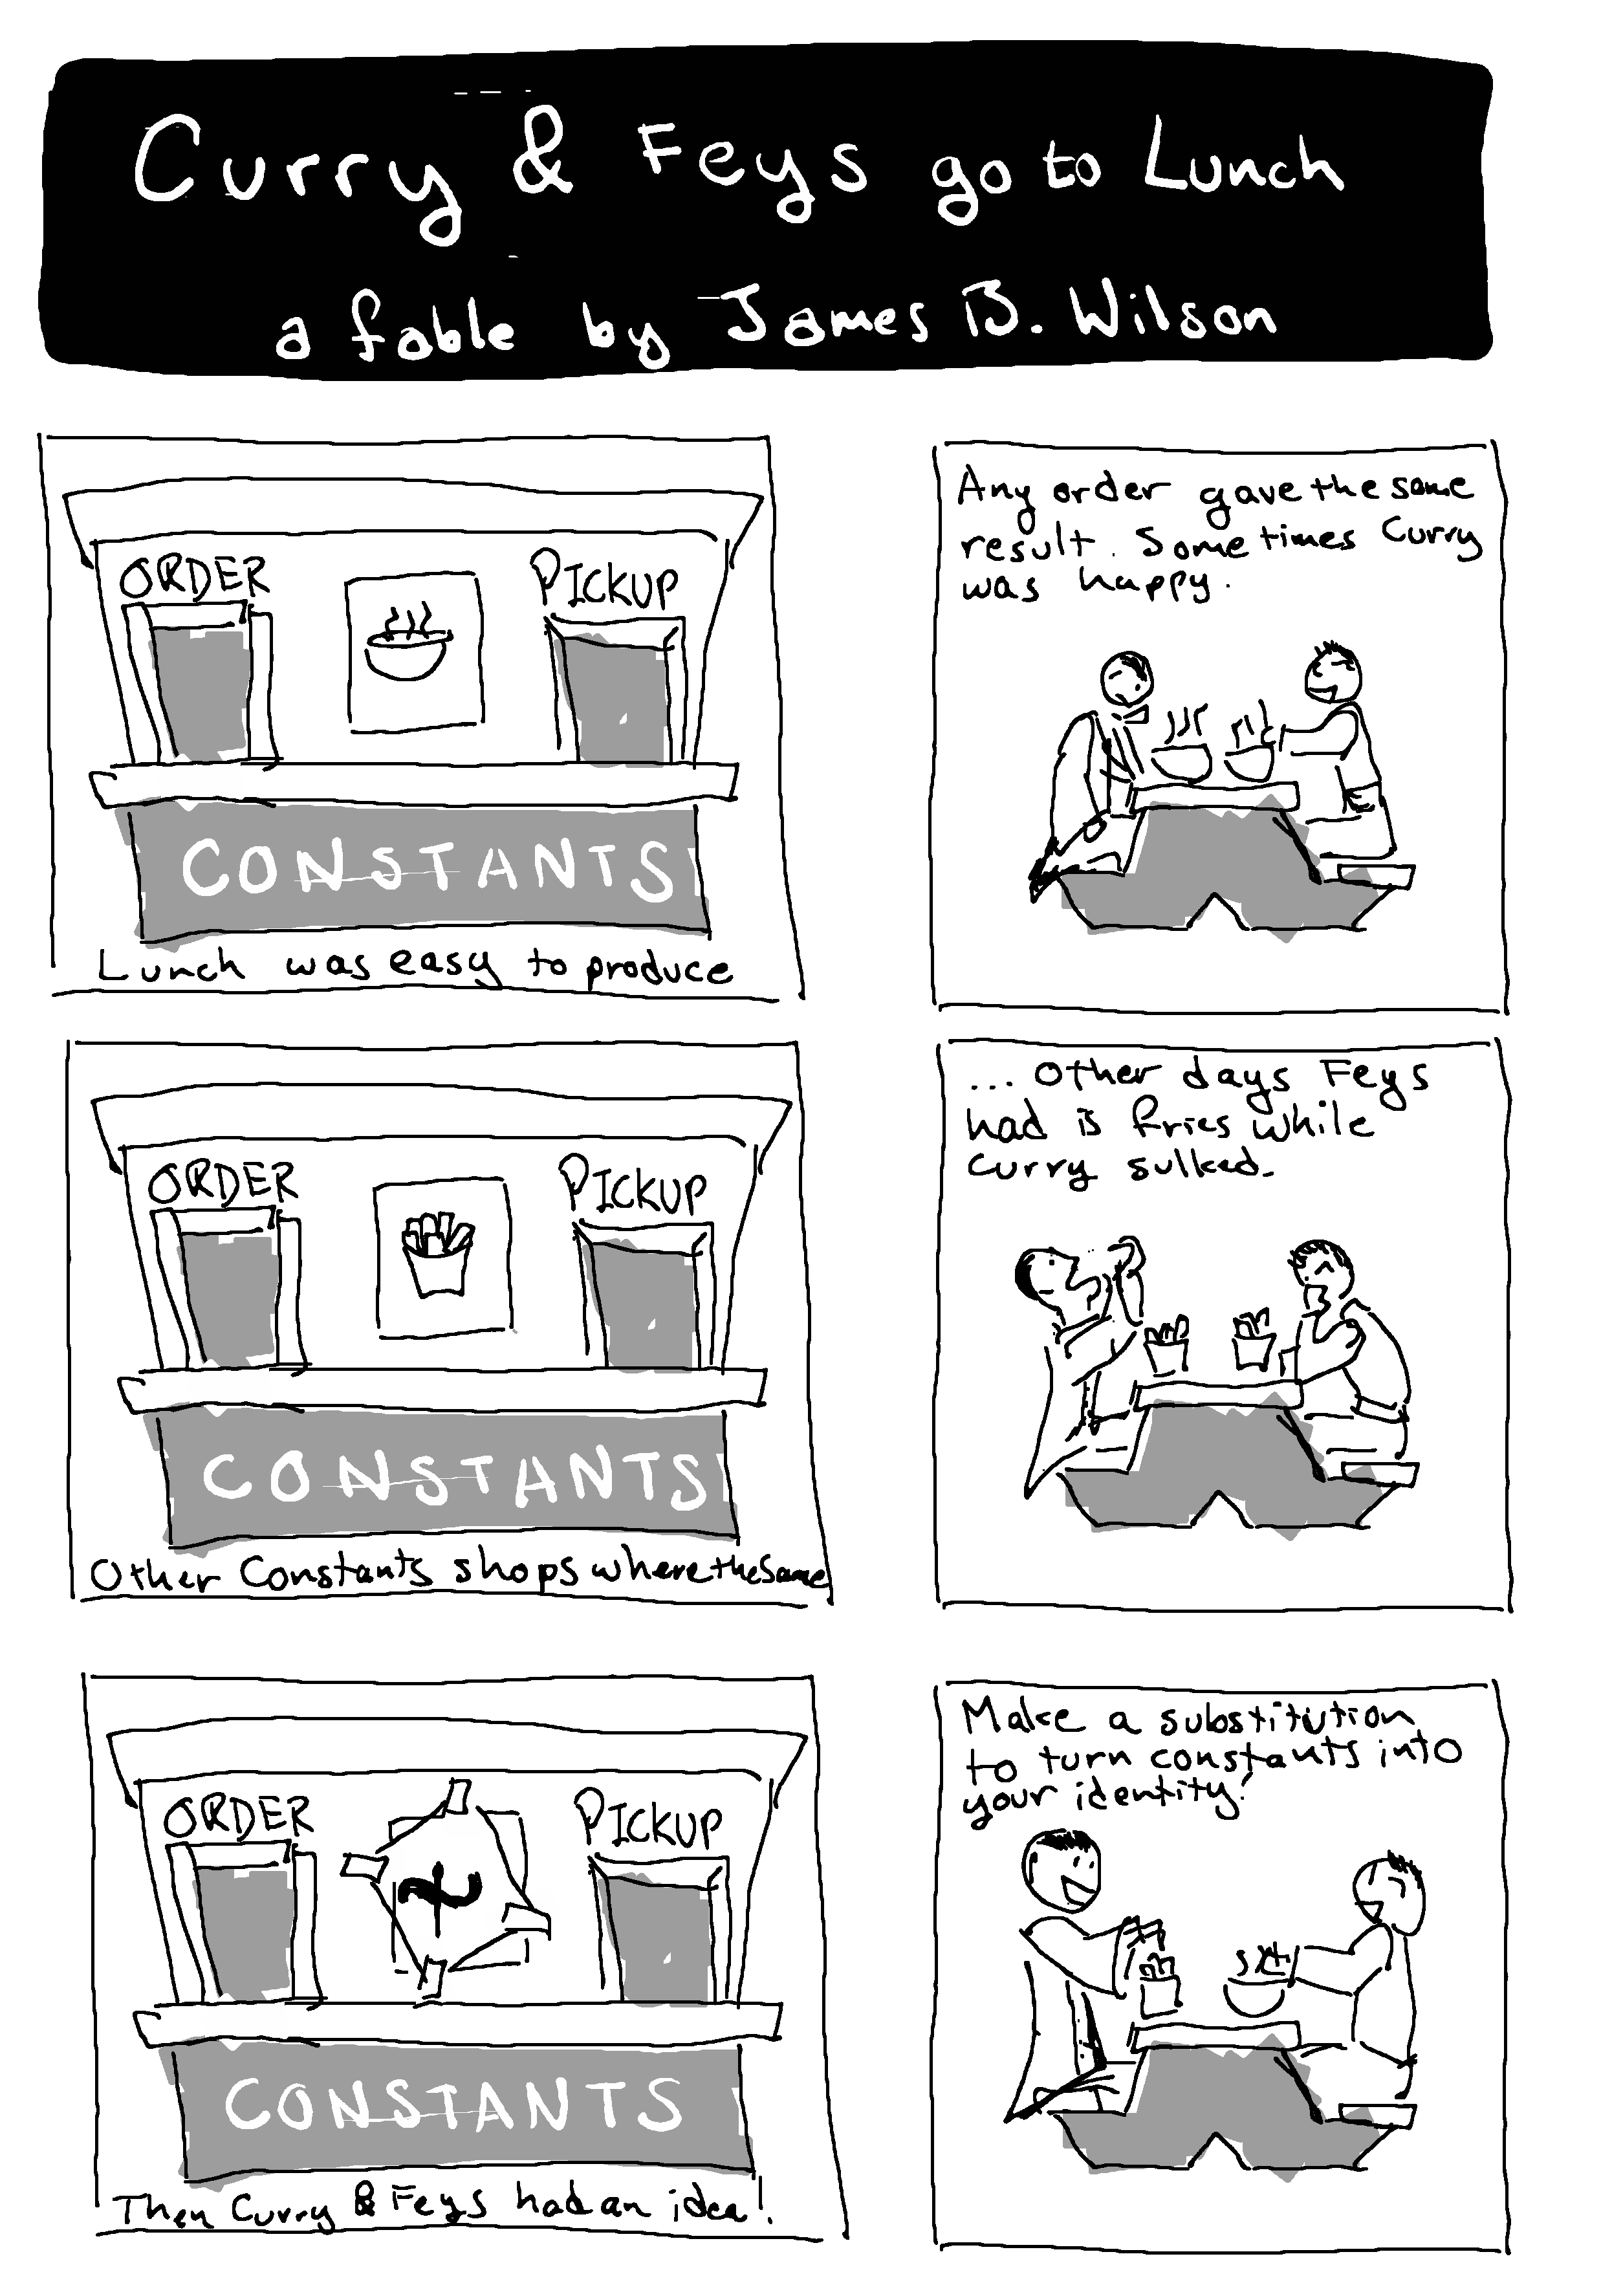
\includegraphics[width=\textwidth]{curry-feys.png}

\chapter{Substitution and Operators}

\chapter{Grammar school}

\begin{quote}
``... small number
of symbols and their grammar are enough to capture the huge
variety of equations...''
\end{quote}

The point of a variable is to replace it.  So in the formula 
$x(x+3)^2$ replacing $x$ for $7$ gives us $7(7+3)^2$.  
Yet even in the land of pure algebra where every symbol is variable it is absurd to
replace $+$ for $7$ to get $x(x73)^2$.   There is restraint in the substitution
of algebra built into what makes something an algebraic formula. When we pull 
on this thread we unravel an expansive relationship between free algebras and induction
and their role in computation.
% \medskip

% It is none other than grammar.

Consider how we know what to do when   
calculating $7(7+3)^2$.  For some of us a mnemonic springs to mind
(\emph{Please Excuse My Dear Aunt Sally}) or an acronym (PEMDAS).
These both unwind to tell us: Parenthesis Exponents Multiplication Division Addition Subtraction
in that order. This meandering thought process somehow elucidates how to read a formula. 
It gives the symbols complex structure that 
can be visualized with the following comic strip.
\begin{center}
    \begin{tikzpicture}[yscale=0.65]
        \node (A) at (0,0) {\begin{tikzpicture}[yscale=0.75]
        \node (f) at (0,0) {$7(7+3)^2$};
        \node[below of=f,scale=0.75] {$\times$};
        \node (x1) at (-1,-2) {$7$};
        \node (sqrt1) at (1,-2) {$(7+3)^{2}$}; 
        % \node[below of=sqrt1,scale=0.75] {$\circ$};
        \node (su) at (1.5,-3) {\textasciicircum $2$};
        \node (u) at (1,-4) {$7+3$};
        \node (x2) at (0,-6) {$7$};
        \node[below of=u,scale=0.75] {$+$};
        \node (three) at (2,-6) {$3$};
        % \node (x3) at (0,-8) {$x$};
        % \node (x4) at (2,-8) {$x$};
        % \node[below of=x2,scale=0.75] {$\times$};

        \draw[-] (f) -- (x1);
        \draw[-] (f) -- (sqrt1);
        % \draw[-] (sqrt1) -- (su);
        \draw[-] (sqrt1) -- (u);
        \draw[-] (u) -- (x2);
        \draw[-] (u) -- (three);
        % \draw[-] (x2) -- (x3);
        % \draw[-] (x2) -- (x4);

    \end{tikzpicture}};
    
    \node[right of=A,xshift=3cm] (B) {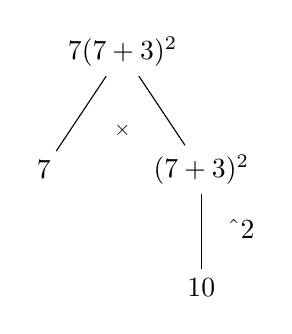
\begin{tikzpicture}[yscale=0.75]
        \node (f) at (0,0) {$7(7+3)^2$};
        \node[below of=f,scale=0.75] {$\times$};
        \node (x1) at (-1,-2) {$7$};
        \node (sqrt1) at (1,-2) {$(7+3)^{2}$}; 
        % \node[below of=sqrt1,scale=0.75] {$\circ$};
        \node (su) at (1.5,-3) {\textasciicircum $2$};
        \node (u) at (1,-4) {$10$};

        \draw[-] (f) -- (x1);
        \draw[-] (f) -- (sqrt1);
        % \draw[-] (sqrt1) -- (su);
        \draw[-] (sqrt1) -- (u);

    \end{tikzpicture}};
    
    \node[right of=B, xshift=3cm] (C) {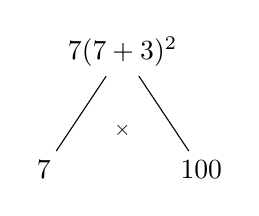
\begin{tikzpicture}[yscale=0.75]
        \node (f) at (0,0) {$7(7+3)^2$};
        \node[below of=f,scale=0.75] {$\times$};
        \node (x1) at (-1,-2) {$7$};
        \node (sqrt1) at (1,-2) {$100$}; 

        \draw[-] (f) -- (x1);
        \draw[-] (f) -- (sqrt1);

    \end{tikzpicture}};
    \node[right of=C,xshift=1cm] {$700$};

    \draw[thick] (A.north east) -- (A.south east);
    \draw[thick] (B.north east) -- (B.south east);
    \draw[thick] (C.north east) -- (C.south east);
\end{tikzpicture}
\end{center}
These step-by-step instructions start at the leaves $7$ and $3$ and join them as $7+3$ (computing $10$),
then the next step is to square (now $100$), then multiply by $7$, we reach $700$.
In hindsight, PEMDAS taught children a complicated form of induction.

\subsection{Induction \& Grammar}
You may have been taught induction through stories of falling 
dominos.  Good.  But what if induction was more like what we just did, climbing?
The domino illustration could bottle up the experience of climbing stairs.  
Now we climb trees and maybe mountains.
Setting up this induction was nothing more than a fragment of text but 
read through the lens of a grammar, e.g.\ PEMDAS, it came into a full form
as steps for recursion.

Parsing grammars in natural language is not always clarifying.  A simplistic
English grammar will often parse into cycles.
\begin{center}
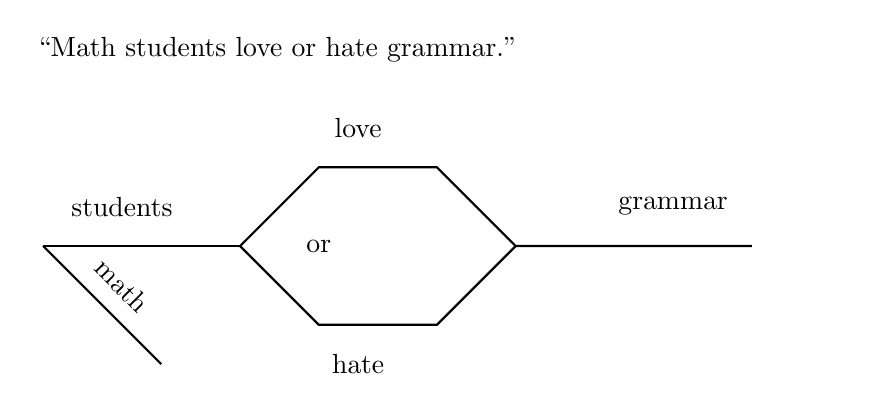
\begin{tikzpicture}
    \node[text width=4in] at (1,2) {``Math students love or hate grammar.''};
    \node at (-3,0) {students};
    \node[rotate=-45] at (-3,-1) {math};
    \node at (-0.5,-0.5) {or};
    \node at (0,1) {love};
    \node at (0,-2) {hate};
    \node at (4,0) {grammar};

    \draw[thick] (-4,-0.5) -- ++(2.5,0);
    \draw[thick] (-4,-0.5) -- ++(1.5,-1.5);
    \draw[thick] (-1.5,-0.5) -- ++(1,1) -- ++(1.5,0) -- ++(1,-1) -- ++(3,0);
    \draw[thick] (-1.5,-0.5) -- ++(1,-1) -- ++(1.5,0) -- ++(1,1);

\end{tikzpicture}
\end{center}
So our inductive climbs may one day need many routes, even go in cycles.
Fortunately, evaluating a formula has a precise algorithm without ambiguity. The
reason is that we had a rooted tree.  Trees have unique paths between any two
vertices. So if we start at the leaves we have a unique direction to reach the
root. 



\index{context-free}
That we got a tree in math formulas means we have a rather boring grammar, 
what Chompsky's \emph{Syntactic Structure} calls
\emph{context-free} grammars.\footnote{
    If an algebraist starts a talk with a story that ``...It was thought  all natural 
    languages were context-free until some obscure dialect in the alps or Africa was found...'', 
    then tune out until they return to equations.  
    Linguist never had such illusions. Even english is not context-free, read  James Higginbotham.} 
Don't be too disheartened.  Virtually every programming language has a 
context-free grammar and programs can communicate a lot of hefty ideas. 

\begin{quote}
    \textbf{Complex inductions can be specified by grammar.}
\end{quote}

\section{Free substitution}\index{variable}\index{substitution}
As a start, it matters first to admit that functions do not need 
domains.  Surprised? Disagree?    Suppose in high school we asked 
a student to  explore
\[
    f(x) = \frac{\sqrt{e^x-1}}{x^2-x-6}.
\]
We might pass this to a graphing calculator, or try some inputs. Along the way
we see the calculator gives up on plotting values $x=(-\infty,0],3$.  Yet, all
we gave it was the formula without prior knowledge of these conditions.  
Be honest with yourself, wouldn't you have thought you could use some of 
those numbers until you tried it as well?

It is a general reality that attention to domains is an afterthought to an
algebra problem, not a forgoing assumption.  In fact if we explore inputs
outside the domain we might discover they are not so bad.  Many of them would
simply lead to complex numbers, and we might arrange for that eventuality.  
What we really have is an understanding of functions and to that we may later 
add aspects such as domains and codomains to study them in restricted ways.

So what is a function if we have not got domains and codomains with which to start?

Let us take seriously the idea of simple substitution: replacing $x$ for something else.
Start with something familiar like substituting $4$ for $x$, but to make 
it sporting use Roman numerals.
\[
    f(IV) = \frac{\sqrt{e^{IV}-1}}{IV^2-IV-6}.
\]
This is hideous but at the same time it remains appropriate, we can interpret 
$f$ as applying to $4$ however we choose to represent it.  The same happens with 
the concept of the variable $x$, we can rename it.
\[
    f(t) = \frac{\sqrt{e^{t}-1}}{t^2-t-6}.
\]
The way we know how is wrapped up in the fact that we know 
in principle how to replace $x$ by any symbol, say $x\leftrightarrows \clubsuit$
\[
    f(\clubsuit) = \frac{\sqrt{e^{\clubsuit}-1}}{\clubsuit^2-\clubsuit-6}.
\]
If we need to make sense of expressions like these we might call $\clubsuit$ 
a ``place holder'' for some yet undeclared explanation.  Yet on the otherhand 
I think it best to think of this more similar to  $f(-1)$, which, if used 
would lead to the temporary absurdity of a negative inside a square-root.
It would be unknown perhaps but not disqualifying.

This type of substitution is completely sound.  To make this clear let us agree 
to a notation simplification.  In much of writing there is a single direction 
to read, e.g.\ left to right.  In mathematics however we can place symbols 
all around and take in that information in any order if not all at once.
\begin{align*}
    \frac{x+2}{x-1} \qquad (x+1)^{x-9} \qquad \begin{bmatrix} x-1 & x+1\\ x-3 & x \end{bmatrix}.
\end{align*}
So let me ask that when you see such formulas you decide on a sequence in your own mind 
on how to 
read it, for example $(x+1)^{x-9}$ could be serialized as 
\begin{center}
    \code{(x+1)^(x-9)}
\end{center}
In this way everything we write can be discussed as a string $M_1 M_2\cdots M_{\ell}$
of small strings $M_i$, even if in reality the layout is more interesting.

With this notion of string, let us begin with the general case where everything 
can be replaced.  This means the atoms of the decomposition are restricted to an
alphabet we call ``variables''. That is all it means to be a variable: you are a
variable if you are in the alphabet of variables.  

\begin{definition}[Pure substitution]
    Given strings $M$ and $N$, and a variable $x$, to replace $x$ in $M$ by $N$ ,
    denoted here as $M[x\leftrightarrows N]$ by follow these rules.
    \begin{description}
        \item[Free.match] $x[x\leftrightarrows N]\defeq N$.
        \item[Free.other] $M[x\leftrightarrows N]\defeq M$ if $M$ is in the variables alphabet (and 
        because we already will have intercepted the case $M=x$ in the above case we know $M\neq x$).
        
        \item[Free.recurse] $(LM)[x\leftrightarrows N]\defeq L[x\leftrightarrows N]M[x\leftrightarrows N]$
    \end{description}
\end{definition}

A word on notation.  Some authors us $M[N/x]$ or $[N/x]M$ in place of $M[x\leftrightarrows N]$
but that notation runs into problems in algebra which has other intentions for `/'.
The Walrus $\defeq$ is notation for naming also called ``assignment''.
\begin{quote}
    ``James $\defeq$ the author.''\\
    ``N is 4.''
\end{quote}
On the left of $\defeq$ should be an as yet unused string of symbols and on the right 
one already known to the context.  Once we have named $M\defeq N$, then 
everywhere we use $M$ it is understood that we intend it to be $N$.
In this way $M=N$ because they are used interchangeably.  We say that 
$M$ is \emph{judgementally} (or \emph{nominally}) equal to $N$, meaning that there is 
nothing to be decided, it is so by declaration.\index{judgemental equality}\index{nominal|see{judgemental}}

\begin{remark}{Replace variables don't assign them}
    There is a widely used abbreviation $x\defeq 2$ used 
    in place of $x[x\leftrightarrows 2]$ popular especially to programs.  
    It is common to encounter arguments shaped like the following.  Given:
    \begin{align*}
        M & \defeq x+3 & N & \defeq 2x
    \end{align*}
    ``Assign $x \defeq 2$ to find...''
    \begin{align*}
        M  & = 2+3 =5 & N & = 2\cdot 2 =4
    \end{align*}
    Strictly speaking, $x$ is in the variable alphabet and $2$ in the constant 
    alphabet so no amount of ``assignment'' can turn one into the other.
    The more accurate description is the following:
    \begin{align*}
        % M & \defeq x+3 & N &\defeq 2x\\
        M[x\leftrightarrows 2] & = 2+3=5 & N[x\leftrightarrows 2] & = 2\cdot 2=4.
    \end{align*}
    Confusing replacement with assignment leads eventually to confused 
    results.  For example, if later we reassign $x\defeq 7$ then $M=10$ not 5.
    To unwind this requires that we sequence all uses of $M$ and think of $M$ 
    ``at time/step 1, 2, ...''.  Retaining the substitution notation is 
    on the other hand always accurate.
\end{remark}



% This type of substitution got us into trouble, after all $(K_c(x)=x)[c\leftrightarrows x]$
% would become $x$.



% It will shock no one that given a formula
% \[
%     f(x) = \frac{x}{\sqrt{x^{2}-\frac{5}{3}x}}
% \]
% it is possible to replace $x$ by any symbol I like.  
% Here I swapped $x\leftrightarrows 2$:
% \[
%     f(2) = \frac{2}{\sqrt{2^2-\frac{5}{3}2}}=\frac{2\sqrt{3}}{\sqrt{2}}.
% \]
% To be cute I next used the Roman Numeral $x\leftrightarrows III$
% \[
%     f(III) = \frac{III}{\sqrt{III^2-\frac{5}{3}III}} = \frac{III}{II}.
% \]
% While it is unusual to work with Roman numerals this was in fact 
% valid.  To give it meaning we had to consult some interpretation 
% of Roman numerals as numbers and calculate in that notation. 
% As that worked what about $x\leftrightarrows \clubsuit$:
% \[
%     f(\clubsuit) = \frac{\clubsuit}{\sqrt{\clubsuit^2-\frac{5}{3}\clubsuit}}.
% \]
% At this point we might see this as a step too far.  Perhaps we might observe 
% that $\clubsuit$ is not in the domain.

% To call this ``evaluating $f$'' goes too far.  We truly are erasing 
% one symbol and drawing in another.  To emphasize this, suppose 
% we had not been given ``$f(x)=...$'' but instead this:
% \begin{align*}
%     f(x) 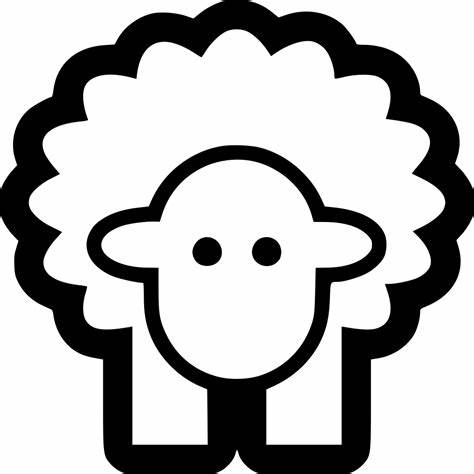
\includegraphics[width=0.5cm]{sheep.jpg} x\sqrt{x^2-x}
%     \qquad 
%     f(\clubsuit) 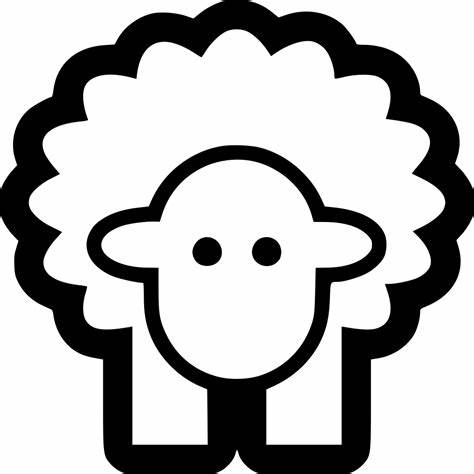
\includegraphics[width=0.5cm]{sheep.jpg}\clubsuit \sqrt{\clubsuit^2-\clubsuit}
% \end{align*}
% The substitution worked just as well and our only concern now is will the sheep eat 
%  the clovers $\clubsuit$.  

% This silly illustration points out that $f(x)=...$ 
% is tempting us to put too many assumptions on what the symbols mean.
% For example you might have thought there was an implied domain of decimal numbers.
% After all square-roots often turn up for decimals.  And yet that cannot be 
% enough motivation because all of us will, if we are honest most of use will on occasion 
% attempt to evaluates such a function at a number that wont make sense long term.


% , and if treated 
% just as symbols our minds may no longer lead us to a misunderstanding.  The locations
% of a fixed symbol are what matter, not the symbol itself.

% Given that location matter, notice that formulas use an array of locations:
% left-right $LM$, e.g.\ $(x+2)(x+3)$; up-down $\overset{L}{M}$, e.g.\ $\frac{x+2}{x+3}$
% on the diagonals $L^M$, e.g.$(x+2)^{(x+3)}$, in three dimensions, e.g. a tensor product $u\otimes v\otimes w$
%     \begin{center}
%         \includegraphics[width=2in,page=26]{Tensor-Product-Def-3D.pdf}
%     \end{center}
% The trouble is that when exploring substitution we want to give a step-by-step 
% description, not including nuances of locations.  So, actual location not-withstanding,
% when we decompose a formula we shall narrow 
% our notation to inline, so $N=LM$ and think of the result as a ``string'' reading 
% left-to-right.

Often in our applications it makes sense to leave some symbols fixed.
For example $0,1,2,3,\ldots$ or the number $\pi$ might not vary in an application.
When this is the case we make a separate alphabet of constants and change substitution 
rules around that alphabet.
\begin{definition}[Applied substitution]
    Given strings $M$ and $N$ with variables or constants, 
    and a variable $x$, to replace $x$ in $M$ by $N$ 
    follow the rules of pure substitution but add the following  base case:
    \begin{description}
        \item[Constant] $c[x\leftrightarrows N]\defeq c$ when $c$ is a constants alphabet. 
    \end{description}
\end{definition}

Towards our earlier point in Chapter~\ref{chp:what-is-algebra}, pure algebra has no constants.


\section{Bound substitution}\index{bound}
With everything said so far we seem no closer to unravelling the paradox 
of the trapped variable.  Following our rules for free substitution and 
Walrus naming, $\CombK{c}(x)\defeq c$ so 
\begin{align*}
    \tag{Nominal equality}
    (\CombK{c}(x))[c\leftrightarrows x] 
    &\quad =\quad c[c\leftrightarrows x]\\
    \tag{Free.match}
    & \quad =\quad x.
\end{align*}
The problem however was not in the symbols, but in what we interpreted them 
to mean.  Recall we tempted ourselves to treat both $I$ and $K$ as operators
and we knew identity operators are not constant operators.

To put a finger on the problem, when we use the Walrus we are giving 
a string a name.  So $f(x)\defeq M$ gives $M$ the name $f(x)$.  
We could just as well have called $M$ by the name $x(f)$ or $xfx$ or 
even ignored $x$ and written $James\defeq M$.  This lead to the substitution 
rules being applied based on nominal reasoning.  Yet, we all know that 
the role of placing $x$ in parentheses is more than naming our operator.
It is meant to identify the correct symbol to play the role of variable.


\subsection{Operator Abstraction}
\index{operator!abstraction}\index{operator!naming}
We need to narrow how we use strings so that substitution behaves 
like in should in operators.  (Recall ``abstraction'' means to restrict reason by rules.)
We signal this abstraction by by writing:
\begin{equation}
    \tag{Operator Abstraction}
    x  \mapsto M
\end{equation}
(Historically this is called function abstraction but we are 
attempting to reserve the word ``function'' for the set-based meaning)
To be clear $x$ here must be a variable, that is, from the variable 
alphabet.  $M$ can be any string even one not containing $x$.
Notice we did not  name the operator `$f$' or something related, 
this is in a real sense an \emph{anonymous operator}.  To 
name a operator we can use $f\defeq (x\mapsto M)$ 
but we almost always abbreviate this to $f:x\mapsto M$.

Our examples so far include:
\begin{align*}
    \CombI:x & \mapsto x, &
    \CombK{c}:x & \mapsto c, &
    \CombK{}: c & \mapsto (x\mapsto c).
\end{align*}



The variable set apart as the input is said to
be \emph{bound} to the operator, it now has a specific role to play similar to
how $\forall x.P$  and $\exists x.Q$ bind $x$ into a special roles in propositions.
Variables that do not have special roles are called \emph{free}.  
Historically Church used the notation $\lambda x.M$ to match those 
patterns and for this reason such functions today are called \emph{Churches}, 
only joking, they are called ``lambdas''. 

Note that the special role of $x$ in $x\mapsto M$ is limited to $M$.  We can say
$M$ is the \emph{scope}.   For this reason programs typically refer to bound
variables as \emph{local}.  Now let us extend substitution into lambdas.
\begin{definition}
    Assume an alphabet of variables with the property that it can always increase in number
    (e.g.\ $x_1, x_2,\ldots$).
Given strings $M,N$ and variables $x,y,\ldots$,
\begin{description}
    \item[Bound.match] $(x\mapsto M)[x\leftrightarrows N]\quad \defeq\quad (x\mapsto M)$
    \item[Bound.trapped]
    if $x$ is a free variable in $M$ and $y$ is a free variable in $N$ then 
    \[ 
        (y\mapsto M)[x\leftrightarrows N]
        \quad \defeq\quad 
        \bigl(z\mapsto (M[y\leftrightarrows z][x\leftrightarrows N])\bigr)
    \]
    where 
    $z$ is a variable distinct from any in $M$ and $N$ (which exists 
    as there are unbounded numbers of variables);

    \item[Bound.other] $(y\mapsto M)[x\leftrightarrows N]\quad \defeq\quad 
    (y\mapsto M[x\leftrightarrows N])$.
\end{description}
\end{definition}

\subsection{Operator Application}
The purpose of binding a variable is to control substitution but it may seem 
with rules like $(x\mapsto M)[x\leftrightarrows N]\defeq (x\mapsto M)$ lead 
us to never actually evaluate an operator.  To the contrary we are simply forcing 
ourselves to explicitly declare evaluation as a step, a computation, which 
very well may require work and alter our data.  This is done with a \emph{reduction}
denoted by $\leadsto$.
\begin{description}
    \item[$\alpha$-reduction] given variables $x$ and $y$, with $y$ not free in $N$,
    \[(x\mapsto M)\quad \leadsto_{\alpha}\quad (y\mapsto M[x\leftrightarrows y]),\]
    which simply renames the variable $x$.

    \item[$\beta$-reduction]
    $(x\mapsto M)N \quad \leadsto_{\beta} \quad M[x\leftrightarrows N]$, which replaces all (free)
    instances of $x$ in $M$ with $N$.  This is the main tool, it is \emph{evaluation},
    also called \emph{application}.
    
    \item[$\eta$-reduction]
    $(x\mapsto M)\quad \leadsto_{\eta} \quad M$, which unbinds the variable $x$.
\end{description}
For a combination of any three of these reductions we write $\leadsto$ unadorned.

Reverting temporarily to the notation $f(x)\defeq \ldots$, the $\alpha$-reduction rule
is what makes the following to operators ``the same''.
\begin{align*}
    f(x) &\defeq  \frac{\sqrt{e^x-1}}{x^2-x-6}
    & 
    f(t) &\defeq  \frac{\sqrt{e^t-1}}{t^2-t-6}
\end{align*}
More precisely
\begin{align*}
    f&:x\mapsto \frac{\sqrt{e^x-1}}{x^2-x-6}\\
    f & \leadsto_{\alpha} \biggl(t\mapsto \biggl(\frac{\sqrt{e^x-1}}{x^2-x-6}\biggr)[x\leftrightarrows t]\biggr)\\
      &  = \biggl(t\mapsto\frac{\sqrt{e^t-1}}{t^2-t-6}\biggr).
\end{align*}
While we might express this as ``replacing $x$ by $t$'', our reduction rules
now make it clear that we are also updating the role of the operator abstraction.


Likewise to evaluate $f(x)\defeq \ldots$ at $4$, commonly written as $f(4)$ will 
now strictly speaking mean
\begin{align*}
    f(4) & = \biggl(x\mapsto \frac{\sqrt{e^x-1}}{x^2-x-6}\biggr)4 \\
     & \leadsto_{\beta} \biggl(\frac{\sqrt{e^x-1}}{x^2-x-6}\biggr)[x\leftrightarrows 4]\\
    & =\frac{\sqrt{e^4-1}}{4^2-4-6}.
\end{align*}
Key to this reduction is that we end up removing the operator abstraction, i.e.
the relevant ``$\mapsto$'' has been eliminated in our process.  It is no longer
the same string with symbols swapped.  We have applied the operator and so it 
is no longer a operator of this $x$.

As with $\alpha$-reductions, the use of $\eta$-reductions is mostly cosmetic 
but is useful when shortening computations.  We could recover both from
$\beta$-reductions as 
\begin{align*}
    t\mapsto ((x\mapsto M)t) & \leadsto_{\beta} (t\mapsto M[x\leftrightarrows t]).\\
    (x\mapsto M)x & \leadsto_{\beta} M[x\leftrightarrows x]=M.
\end{align*}


These details
gets us out of the trapped variable paradox.
\begin{align*}
    \CombK{} &: c  \mapsto (x\mapsto c).\\
    \tag{Nominal equality}
    \CombK x & = (c\mapsto (x\mapsto c))x\\
    \tag{Application}
        & \leadsto_{\beta} (x\mapsto c)[c\leftrightarrows x]\\
    \tag{Bound.trapped}
        & = z\mapsto (c[x\leftrightarrows z][c\leftrightarrows x])\\
    \tag{Free.other}
        & = z\mapsto (c[c\leftrightarrows x])\\
    \tag{Free.match}
        & = z\mapsto x
\end{align*}
So in the end the constant $c$ was replaced by $x$ but at the same time 
the variable that was $x$ is now $z$ so $\CombK{x}:z\mapsto x$ remains constant.

\subsection{Exercises}
\begin{enumerate}
    \item Let $f:x\mapsto x\sqrt{x^-9}$.  Evaluate $f(4)$.

    \item Suppose $f(a/b)=a+b$ as formally abstracted as $f:a/b\mapsto a+b$.  What would $f(1/2)$ be?
    What would $f(2/4)$ be? 

    \item Suppose $f(a/b)=a+b$ as formally abstracted as $f:a\mapsto (b\mapsto a+b)$.  What would $f(1/2)$ be?
    What would $f(2/4)$ be?  

\end{enumerate}

\section{Operations are well-defined}
The most important aspect of functions to preserve is the reliability of evaluation.
\begin{align*}
    x=\acute{x} & \Rightarrow f(x)=f(\acute{x}).
\end{align*}
Do we really believe this now that functions are backed up by nothing more
than technical system of substitution we have come to know as $\lambda$-calculus?


A large part of calculations in algebra take place on structures that 
can be have more than one adequate representation.  You learned this 
already in primary school when you were told or shown that
$1/3$ agrees with $0.\bar{3}$, or that $0.\bar{9}=1$. 



Now that we have described operators we should ask if the answers are 
to be trusted in the way that we trust the result of functions.
There is of course the need to be weary of slights of hand.
Is this an operator?
\begin{align*}
    f\left(\frac{a}{b}\right)\defeq a+b.
\end{align*}
Of course not:
\begin{align*}
    1/2 = 2/4 & \Rightarrow 1+2=f(1/2)=f(2/4)=2+4.
\end{align*}
This is just another warning against putting too much confidence 
in the $f(x)\defeq\ldots$ model.  If we abstracted this would be 
$a/b\mapsto a+b$ and so the entire symbol $a/b$ would be the variable 
not $a$ and $b$ separate.  That would 

The payoff is not so much to avoid paradoxes.  Rather by being precise we arrive
at a tool to describe operators as robustly as their set-based cousin
``functions'' but one that operates on so few mechanics that it can apply almost
any where including structures before and beyond sets (higher logic, categories,
and higher categories).  It is also such a computationally precise encoding that
programs can be made to effect these operators. The one catch is that we cannot
guarantee that operators once applied will come to an end in finite time. That's
a reality taught to us by Turing's Halting Problem.

First we should address when to stop an evaluation.
\begin{definition}
    \begin{itemize}
        \item If $G$ and $F$ are strings and there are strings 
        $G_1,\ldots,G_{\ell}$ such that 
        \[ G=G_1 \leadsto G_2 \leadsto\cdots\leadsto G_{\ell}=F\]
        then write $G\leadsto F$.

        \item if $G\leadsto H$ and $F\leadsto H$ then write $G\betaeq H$.
        In particular $G\betaeq F$ if after renaming variables and doing some reductions 
        they agree.

        \item A formula $F$ is \emph{reduced} when it has no terms where 
        $(x\mapsto M)N$.  
    
    \end{itemize}
    
\end{definition}

\subsection{Confluence and Normal Forms}
\begin{theorem}[Church-Rosser]
    If $L\leadsto_{\beta} M$ and $L\leadsto N$ then there is $O$ such that 
    \[M\leadsto_{\beta} O\qquad N\leadsto_{\beta} O.\] 
    In particular, if $F\leadsto S,R$ where both $R$ and $S$ are reduced,
    then $R\betaeq S$ (that is equal up to possibly renaming a variable).
\end{theorem}

This is the first of many \emph{normal-form} theorems in algebra.
Normal forms are unique representations given after rewriting a formula.


\begin{definition}
    A operator is a sentence in $\lambda$-calculus.
    Evaluating an operator is to apply $\beta$-reductions.
\end{definition}

\begin{corollary}
    If a operator evaluates in finite time then whatever process it uses 
    gives the same answer.
\end{corollary}



It is the job of a programming language to implement a version 
of substitution that follows these rules.  Once done the notation will take 
on the usual character of the programming language but often the notation 
comes close to the mathematical notations.  Here are some popular variations to try.
\begin{center}
    \code{lambda x.x+2}
    \hspace{1cm}
    \code{x => x+2}
    \hspace{1cm}
    \code{x |-> x+2}\\
    \code{func(x)=x+2}
    \hspace{1cm}
    \code{(x)-> {return x+2}}
\end{center} 


So our traditional $f(x)\defeq M$ notation would no be hinting at 
$f:x\mapsto M$ in our notation, and the $f$ here would be naming 
the specific example $x\mapsto M$, which is often helpful.  Yet 
we should not take this correspondence too far since we have already 
seen the ways in which substituting for $x$ in $f(x)\defeq M$ notation 
goes astray.

The first rule Bound.match may at first seem odd.  Aren't we trying to place $x$?
Yes but when we write $x\mapsto M$ we are declaring $x$ as a local variable.  
It is completely meaningless what it is called outside the scope of $M$.
It is the same thing we come to expect when we do things like this:


In some situations the role of bound/local variables is further 
restricted to roles of a decidedly special meaning, for example, as indices that 
run through a range.
\begin{align*}
    \sum_{i=1}^{10} i^2 \qquad \prod_{i\in I}X_i 
\end{align*}
or in code 
\begin{center}
\begin{Pcode}[]
def sum(ns)= {
  x = 0
  for n in ns 
    x = x + n
  x  
}

x = [2,3,4]
sum(x)  // the x outside is not the x inside sum
\end{Pcode}
\end{center}
% 
\section{Basic Grammar}
Admittedly  $\Box+\Box$, $\Box\cdot \Box$, and $-\Box$ indicate where to place 
information but they do not clarify what can be placed in each spot. 
We can add some clarity by clarifying the grammar with more meaningful tags.
For example, 
\begin{center}
    \code{<Matrix> ::= <Matrix> + <Matrix>}
\end{center}
would clarify that for this $+$ the intension was to add two matrices and 
the result will be another.   If we want to be certain that the dimensions 
match we can add this to the grammar.
\begin{quote}
    \code{<Matrix(2,3)> ::= <Matrix(2,3)> + <Matrix(2,3)>}\\
    \code{<Matrix(2,4)> ::= <Matrix(2,3)>  <Matrix(3,4)>}
\end{quote}
This approach becomes somewhat tedious as it depends so visibly on 
constants what will change between applications.  Later we revisit 
this problem with a few better options.


There are two implicit assumptions in what 
we have written.  First, while this definition is recursive we only intend 
that we should place a $+$ between two matrices that already exist.  In this 
way the grammar looks only back in time eventually settling on some constant
matrices.  Otherwise we could end up with some sort of infinite loop that 
never draws to a close.  Recursion that looks back in time to a start point is 
called \emph{primitive recursion}.  The second unexplained assumption is what 
qualifies as a constant matrix, a base case, to start the process off. 
The zero matrix for example would be one option, as would the matrices 
$E_{ij}$ that have $0$ in all position except row $i$ and column $j$ where 
the number is $1$.  If we include rescaling as an option then through 
linear combinations we could specify any matrix in this way.

Later we shall be more formal with grammars but we close we a few more 
demonstrations.
\begin{center}
\begin{Gcode}
<List> ::= cat <List> <List>
<List> ::= <List> + <List>
<A or B> ::= if <Boolean> then <A> else <B>
\end{Gcode}
\end{center}
When we wish to indicate that symbols $x$ have met the requirement to be 
treated as a type say ``matrix'', or ``list'', or ``Boolean'' we 
write $x:Matrix$, $x:List$, $x:Boolean$ accordingly.  We are also 
lenient with the use of popular shorthand such as $\mathbb{N}$ for natural 
numbers.  So $n:\mathbb{N}$ indicates that $n$ is a natural number.
Here are some related demonstrations.
\begin{quote}
    \code{(cat [1,2,3] [4,5,6]):List}.\\
    \code{([1,2,3] + [4,5,6]):\text{List}}.\\
    $\displaystyle 
        \begin{bmatrix} 1 & 0 & 8 \\ 2 & 7 & -1\end{bmatrix}
    + \begin{bmatrix} -1 & 0 \\ 0 & 1 \end{bmatrix}:\mathbb{R}^{2\times 3}$.
\end{quote}


\section*{Conclusion}

The process of replacing one set of symbols for another based on fixed rules 
is known in algebra circles as \emph{rewriting}\index{rewriting}.  Rewriting 
occurs everywhere from the evaluation of operators like we are explore now, 
to multiplying solvable groups, to solving algebraic geometry problems through 
Gr\"obner-Shirshov bases.  The strategies of rewriting evolve with every context 
but most have an arc similar to the one we pursue in this chapter.  Start by 
considering the order in which you rewrite.  Make it a partial order or at 
least a directed graph.  Search for confluence: places where branches meet back
together.  When enough confluence exists look for a reason for finite rewriting 
to reach a normal form---a unique lowest point, subject to the order we introduce.
Finally, when normal form exist the work begins to get that normal form efficiently.
Above all notice how many possible points of failure there are in effective 
rewriting.  As a general intuition treat rewriting as undecideable, but if decideable 
then exponentially hard, but if efficient then it was never rewriting---it was 
linear algebra in bad notation. 